% !TeX root = ../Thesis.tex
\documentclass[../Thesis.tex]{subfiles}
\graphicspath{{\subfix{../images/}}}

\begin{document}

\section{Function inlining in the translation to Petri nets}

In this section, a thorough analysis and motivation for the third design decision
listed at the beginning of the chapter, namely inlining function calls, is presented.

Modeling functions in \acrshort{PN} is a crucial aspect of the translation
because it is the basic unit of the MIR representation.
By representing the functions in the MIR as \acrshort{PN} and connecting them accordingly,
the control flow and data shared between the threads in the program
can be captured in a formal framework.
Afterward, the Petri net is analyzed by a model checker
in order to identify potential deadlocks or lost signals.
This approach is especially useful when working with large and complex systems
that may have many interrelated threads and functions,
where the deadlock situation may not be evident even to an experienced code reviewer.

When translating MIR functions to \acrshort{PN}, one key question that arises is
whether to reuse the same representation for every call to a specific function or
to ``inline'' the corresponding representation every time the function is called.
Expressed differently, each function maps to a subnet
in the final \acrshort{PN} obtained after the translation, i.e.
a connected subgraph formed by the places and transitions
that model the behavior of the specific function.
This smaller part of the net can either be present only once in the \acrshort{PN}
and all calls to this function connect to it,
or be repeated for every instance of a call to the function in the Rust code.

Reusing the same model for every function call can be more efficient,
as the \acrshort{PN} obtained is smaller.
However, this approach can also lead to invalid sequences of markings
that were not present in the original program.
These can be the source of false positives in deadlock detection,
as these extraneous states may lead the program to
incorrect states where the safety guarantees made by the compiler do not longer hold.

On the other hand, inlining the model every time a function is called results in
a larger \acrshort{PN}, which requires more memory and processor time to be analyzed,
but it can also improve the accuracy of the analysis by ensuring
that each function call is represented by a unique Petri net structure
that captures its specific data dependencies in the context
in which the function call occurs in the code.

\subsection{The basic case}

The impact of these subtle details can only
be fully comprehended with an appropriate example.
Therefore, consider first the most simple abstraction of a function call in
the language of Petri nets, formed by a single transition and
two places representing the start and end of the function.
This is seen in Fig. \ref{fig:simplest-function}.
The function call is treated as a black box,
all details are abstracted away in the transition.
We care only about where the function starts and where it ends.

\begin{figure}[!htb]
    \centering
    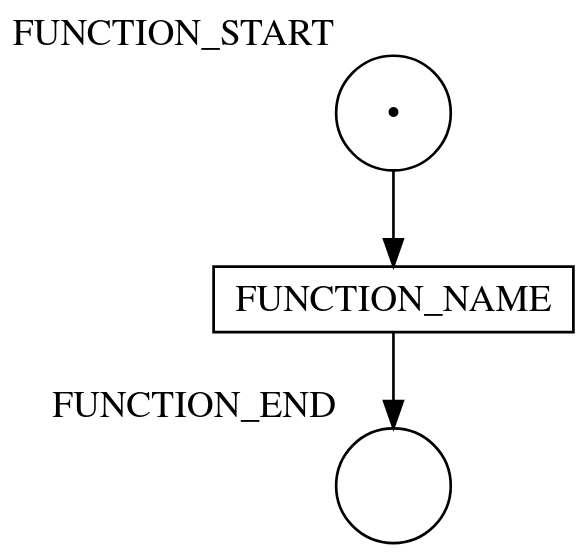
\includegraphics[scale=0.25]{simplest-function.png}
    \caption{The simplest Petri net model for a function call}
    \label{fig:simplest-function}
\end{figure}

Observe now such a function in the context of a Rust program.
Listing \ref{lst:repeated-function-call} shows a simple example
in which one function is called
five times consecutively in a \Rustinline{for} loop.
A possible \acrshort{PN} that models the program
is found in Fig. \ref{fig:repeated-function-call}.
It should be emphasized that
this net does \emph{not} result from a translation of the MIR.
It is a simplification to showcase the difficulties
of dealing with functions called in various places in the code.

\begin{listing}
    \begin{minted}{Rust}
        fn simple_function() {}

        pub fn main() {
            for n in 0..5 {
                simple_function();
            }
        }
    \end{minted}
    \caption{A simple Rust program with a repeated function call}
    \label{lst:repeated-function-call}
\end{listing}

\begin{figure}[!htb]
    \centering
    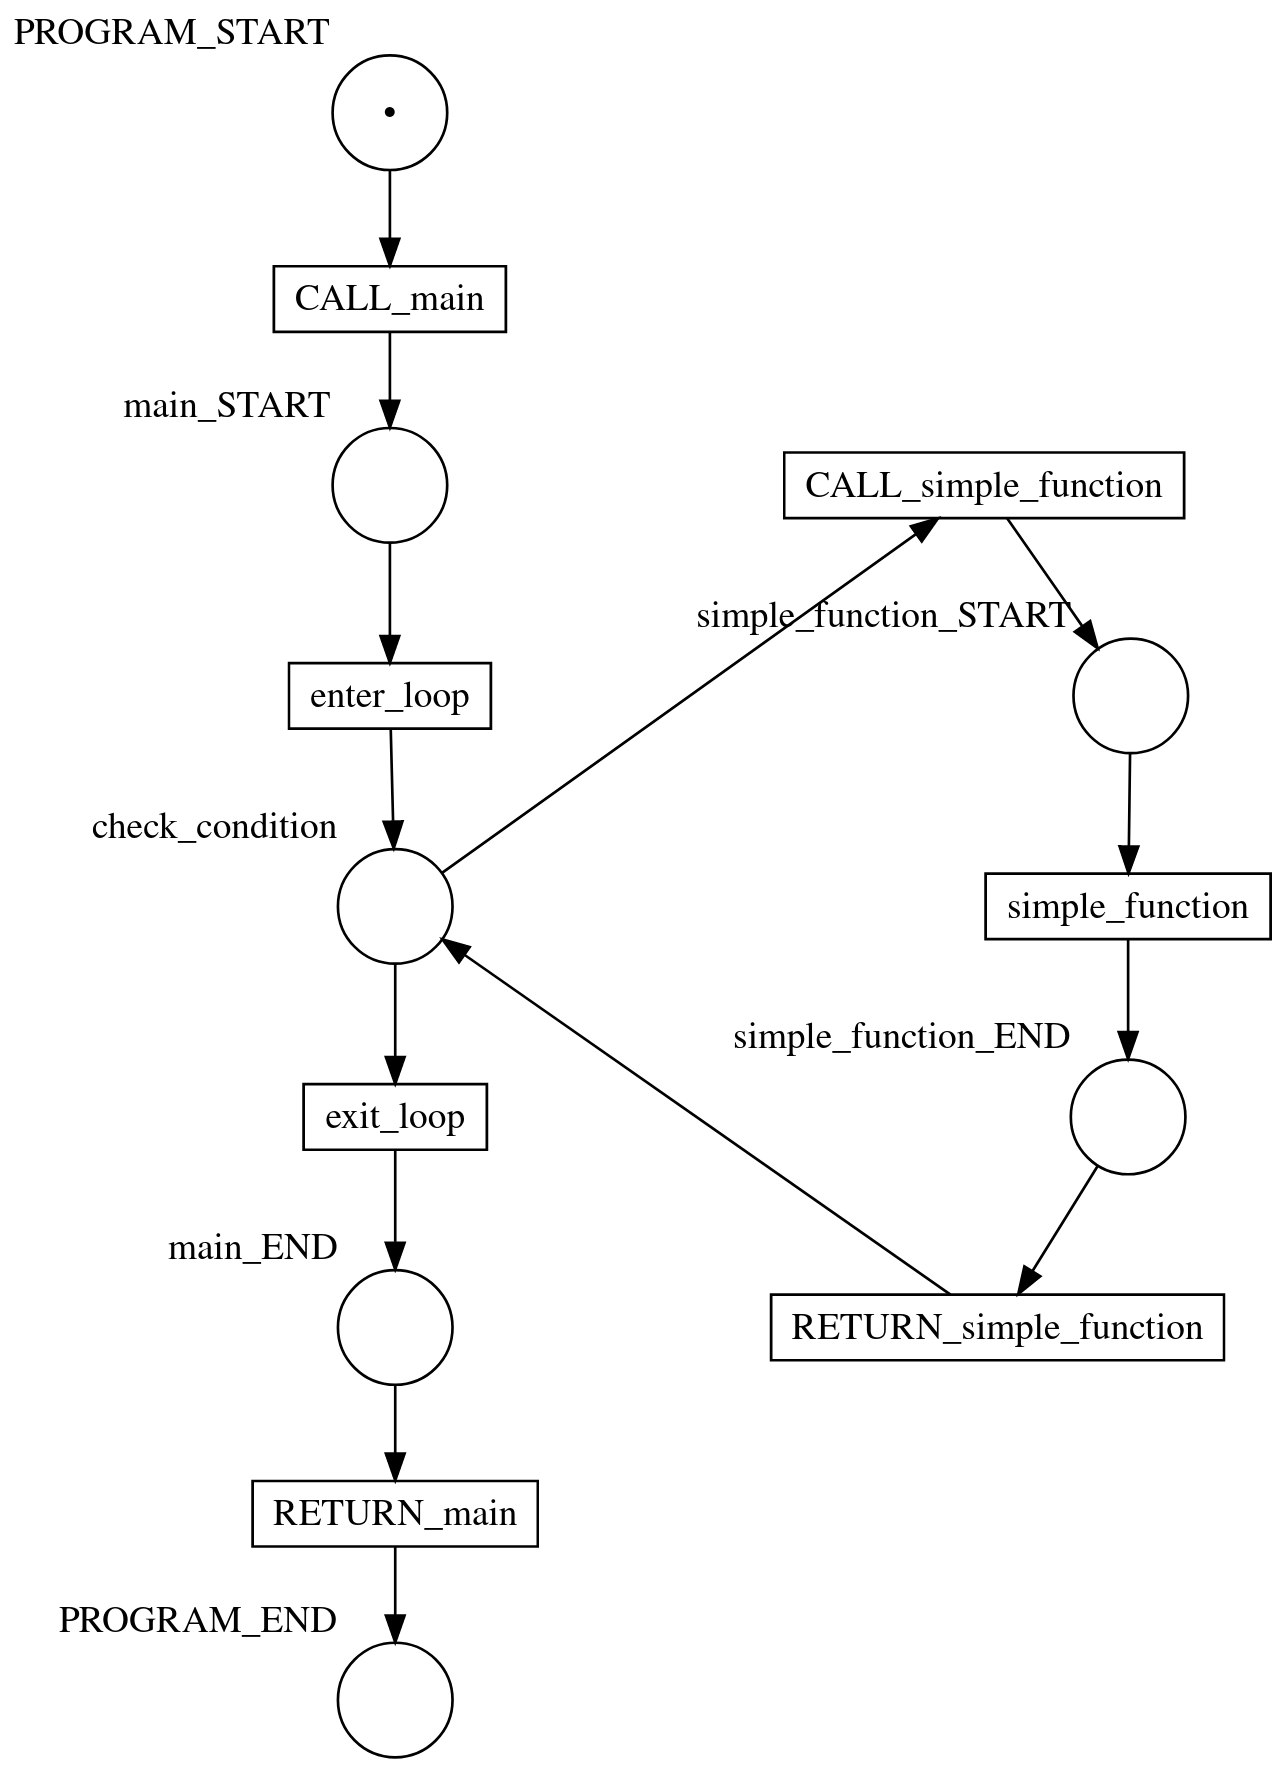
\includegraphics[scale=0.25]{repeated-function-call.png}
    \caption{A possible \acrshort{PN} for the code in Listing \ref{lst:repeated-function-call}
        applying the model of Fig. \ref{fig:simplest-function}}
    \label{fig:repeated-function-call}
\end{figure}

\subsection{A characterization of the problem}

The troublesome scenario has not emerged so far.
It manifests only when a function is called
in at least two different places in the code or,
in simpler terms, the expression \Rustinline{simple_function()} appears twice or more.
Listing \ref{lst:two-simple-function-calls} satisfies this condition
and is designed to exhibit
the extraneous behavior described at the beginning of the section.

\begin{listing}
    \begin{minted}{Rust}
        fn simple_function() {}

        pub fn main() {
            let mut second_call = false;
            simple_function();
            if second_call {
                panic!()
            }
            second_call = true;
            simple_function();
        }
    \end{minted}
    \caption{A simple Rust program that calls a function in two different places}
    \label{lst:two-simple-function-calls}
\end{listing}

As stated before, the first approach to modeling the program consists
in re-using the function model for both calls.
This is shown in Fig. \ref{fig:two-function-calls-incorrect-1}.

\begin{figure}[!htb]
    \centering
    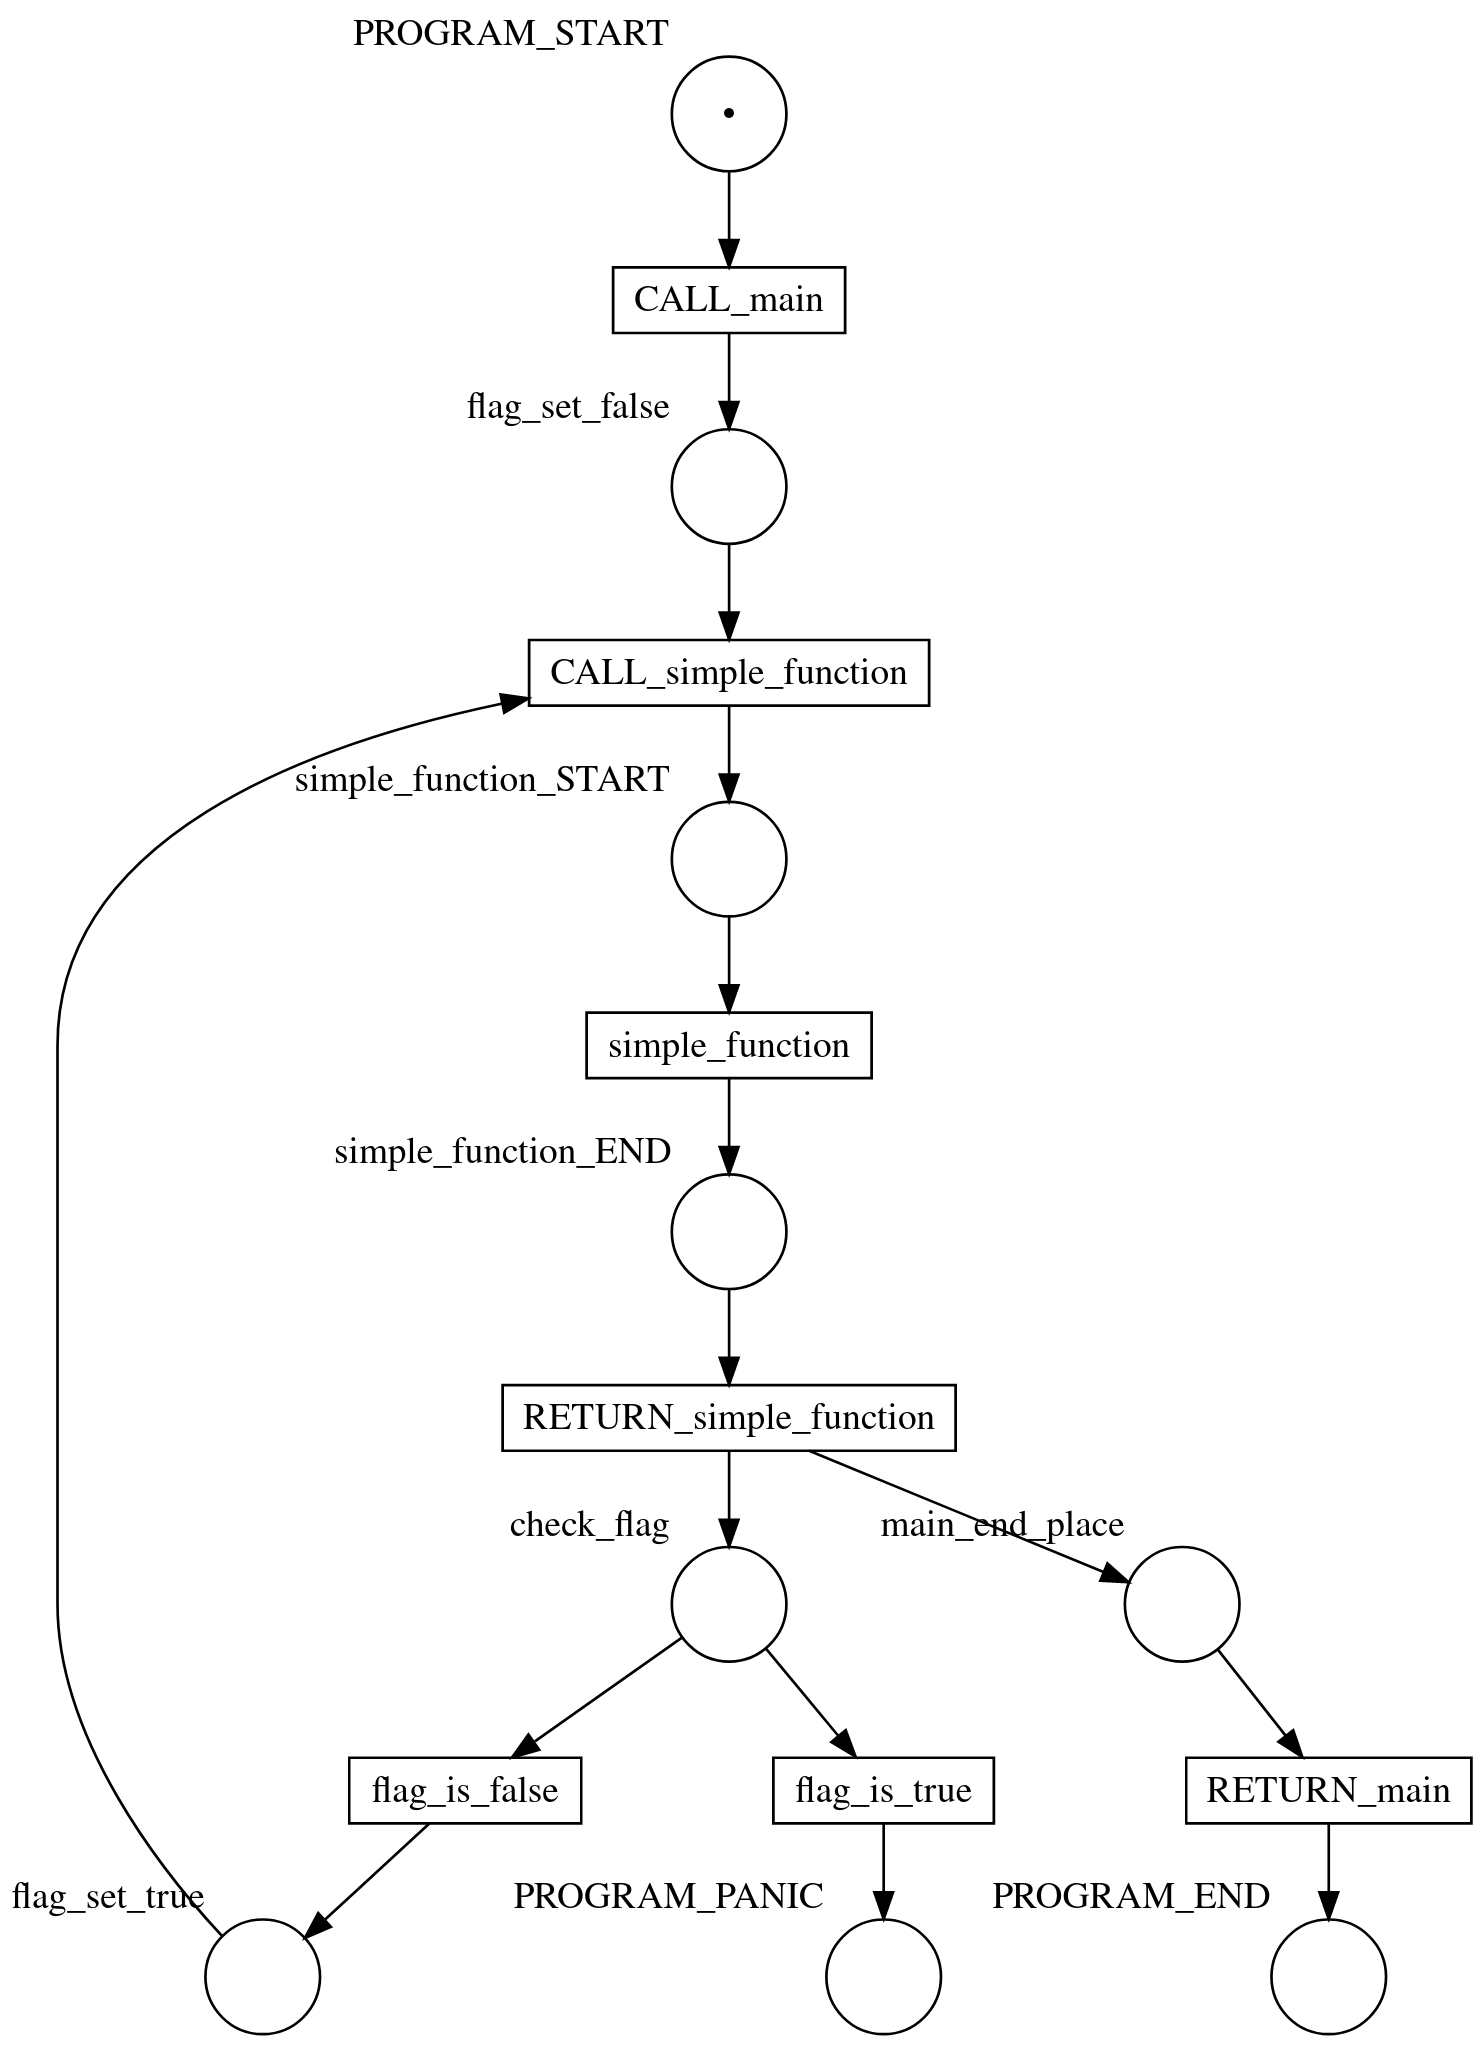
\includegraphics[scale=0.25]{two-function-calls-incorrect-1.png}
    \caption{A first (incorrect) \acrshort{PN} for the code
        in Listing \ref{lst:two-simple-function-calls}}
    \label{fig:two-function-calls-incorrect-1}
\end{figure}

It must be evident to the reader that
the program in Listing \ref{lst:two-simple-function-calls}
never calls the \Rustinline{panic!()} macro and always terminates successfully.
The variable \Rustinline{second_call} is never \Rustinline{true} before line 9.

Yet, the \acrshort{PN} depicted in Fig. \ref{fig:two-function-calls-incorrect-1}.
is conspicuously flawed, making it unsuitable as a model for the program.
The reason is that after firing the transition labeled \texttt{RETURN\_simple\_function}
a token is placed in \texttt{check\_flag} but \emph{also} in \texttt{main\_end\_place}.
The token in \texttt{main\_end\_place} will eventually appear in \texttt{PROGRAM\_END},
which indicates a normal termination of the program.
This is technically correct since we know that the program terminates successfully.

Nonetheless, there are concerning issues regarding the second token.
The token in \texttt{check\_flag} could be consumed either
by the transition \texttt{flag\_is\_false} or \texttt{flag\_is\_true}.
If it is consumed by the latter, a token will be placed in \texttt{PROGRAM\_PANIC},
signaling an erroneous termination of the program.
This is absurd because it means that the program could panic
but also \emph{always} ends normally, as seen in the previous paragraph.

The situation becomes worse if we follow the path of firing \texttt{flag\_is\_false}.
In that case, the token triggers another function call, which is in principle correct,
but nothing prevents it from doing this over and over again.
The result is that an infinite amount of tokens could accumulate
in \texttt{main\_end\_place} or \texttt{PROGRAM\_END}
in the circumstance that, by pure chance,
the transition \texttt{flag\_is\_true} does not fire.

It has become clear that we must discard this model and look for a better solution.
One possibility is to split the transition labeled \texttt{RETURN\_simple\_function}
in two separate transitions depending on the function call order
as illustrated in Fig. \ref{fig:two-function-calls-incorrect-2}.

\begin{figure}[!htb]
    \centering
    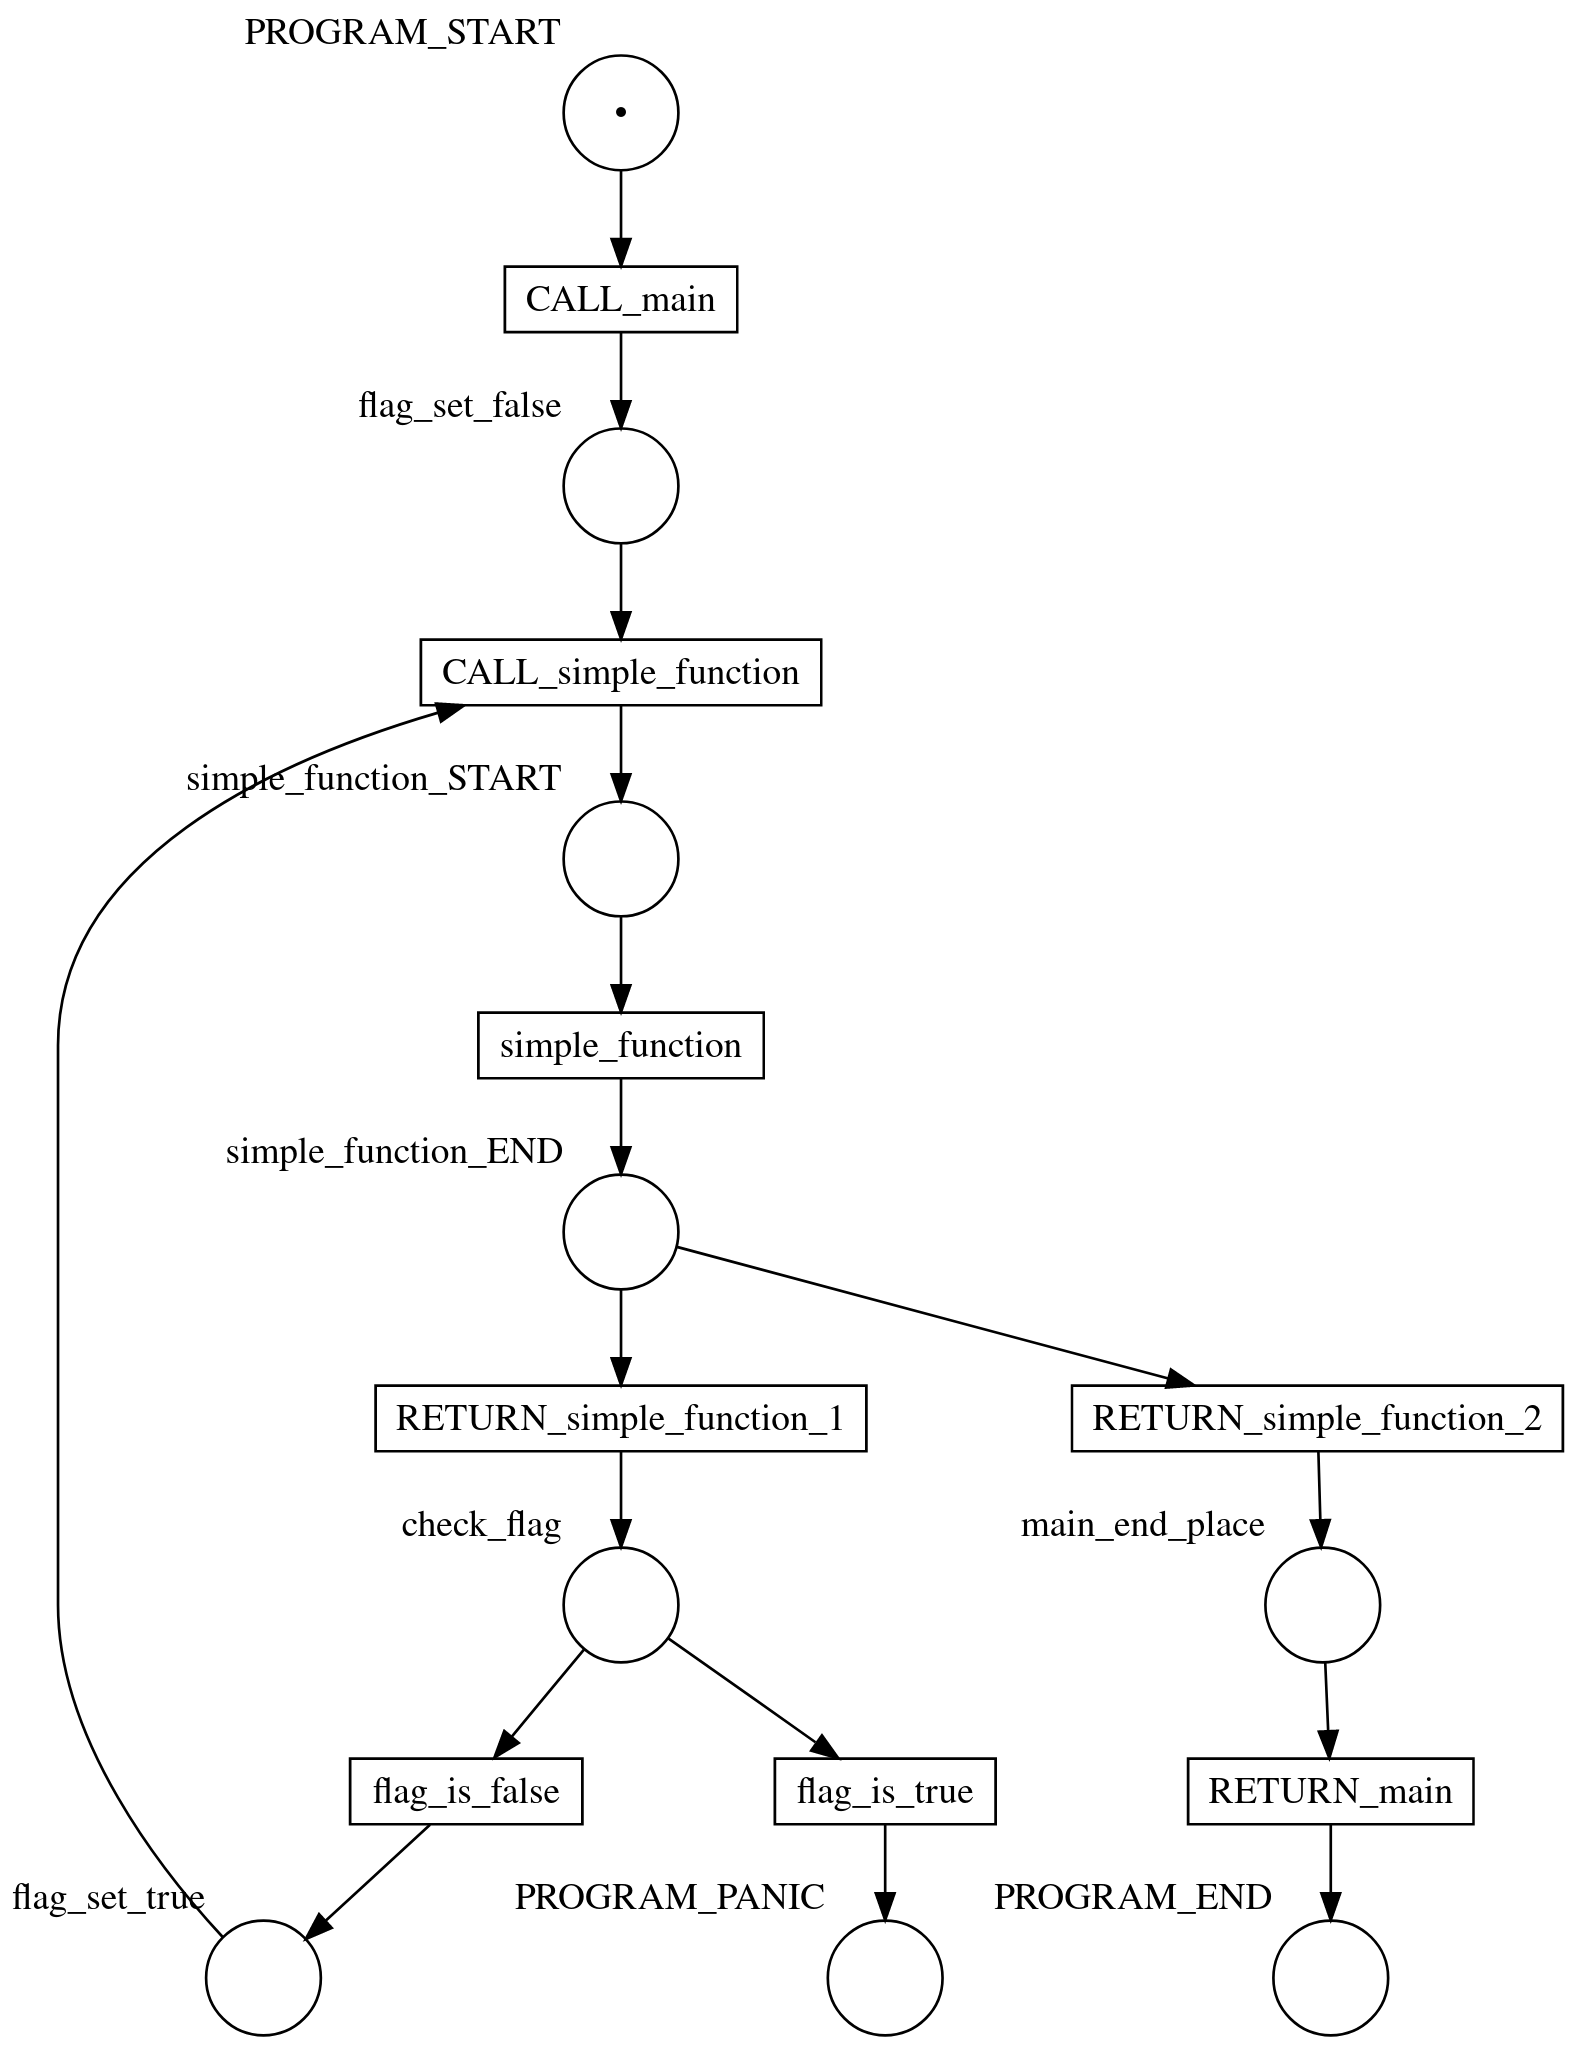
\includegraphics[scale=0.25]{two-function-calls-incorrect-2.png}
    \caption{A second (also incorrect) \acrshort{PN} for the code
        in Listing \ref{lst:two-simple-function-calls}}
    \label{fig:two-function-calls-incorrect-2}
\end{figure}

This second attempt unfortunately comes with its own set of extraneous states.
First, the program may now exit after calling the function only once.
Nothing prevents the transition \texttt{RETURN\_simple\_function\_2} from firing first.
This is equivalent to saying that the execution flow jumps
from line 5 to line 11 in Listing \ref{lst:two-simple-function-calls},
which is obviously not a property present in the original Rust code.

On the other hand, the problem of the infinite loop persists.
The \acrshort{PN} may continue firing indefinitely as long as
\texttt{flag\_is\_true} and \texttt{RETURN\_simple\_function\_2} do not fire.
There is no guarantee that the transitions fire in a specific order.
As seen in Sec. \ref{sec:transition-firing},
the transition firing is non-deterministic.

Having observed this, we turn our attention to the other approach to modeling
function calls: Inlining the \acrshort{PN} representation.

\end{document}